\section{The Operational Situation}

This section will review the Operational Situation of the Battle of Cowpens.  It
will place the battle within the context of the campaign.   For the purposes of
this section, the Southern Campaign began with the British forces invading South
Carolina in February 1780 and this section will conclude January 16, 1781 just
prior to the Battle of Cowpens.

The British plan in the Southern Campaign and its objectives were conceived by
Lord Germain and embraced by Sir Henry Clinton.  First, the British Army would
seize Charleston.  Next, it would raise Loyalist militia forces to gain control
of South Carolina and then North Carolina.  Finally, they were to destroy the
Continental Army of the Southern Department and end all forms of rebellion.

In order to achieve its Southern Campaign objectives, the British Army required
the raising of Loyalist militias.  The idea was for the British Army to gain
control of new areas as they moved inland from the coast.  As they gained
control of an area, Loyalists militias would assume the responsibility of
maintaining security and lines of communication as the British Army progressed.
From lessons learned in the North, “the British had discovered that Loyalists
would only muster when regular British forces were on hand to protect them”
\cite[p.43]{woodward_comparative_2002}.

\begin{figure}[h]
%\begin{wrapfigure}{r}{0.5\textwidth}
\begin{center}
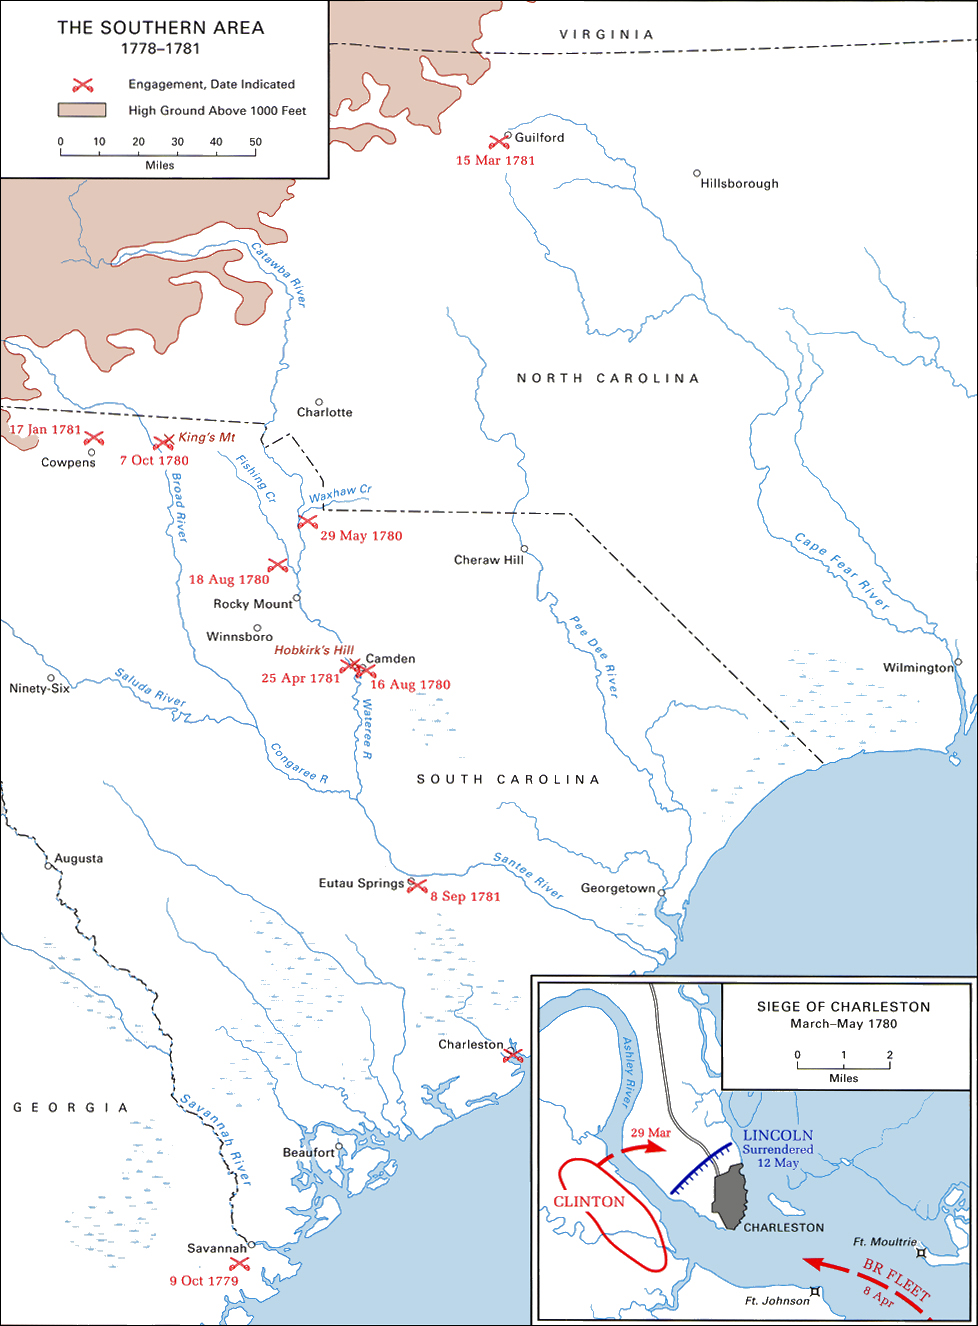
\includegraphics[height=5in]{gfx/Nicholson1}
\end{center}
\caption{The Southern Area of Operations \cite[Map 10, p. 91]{stewart_2005}}
\label{Nicholson1}
%\end{wrapfigure}
\end{figure}

In February of 1780, General Henry Clinton’s force consisting of 10,000 soldiers
and supported by 5,000 sailors landed off Charleston, South Carolina
\cite[p.6]{weigley_partisan_1970}.(See Fig. \ref{Nicholson1})
In response, Major General Benjamin Lincoln decided to defend the city of
Charleston.  General Lincoln’s force consisted of about 2,650 Continentals and
2,500 South Carolina militiamen \cite[p.6]{weigley_partisan_1970}.  Lincoln’s
force was inadequate for the defense; his decision to stay and defend may have
been more politically motivated than tactically thought out.  On May 12, 1780,
General Lincoln surrendered after a prolonged siege.  Virtually all the
organized American military forces in South Carolina had been wiped out.  The
seizing of Charleston allowed the British Army to achieve their first campaign
objective almost immediately.  Charleston allowed for a “good port and base from
which to mount their Southern Campaign” \cite[p.22]{woodward_comparative_2002}.

\begin{figure}[h]
\begin{center}
\includegraphics[height=5in]{gfx/Nicholson2}
\end{center}
\caption{Overview of Southern Theater of Operations 1778-1781 \cite[Tab D, Map 1]{rauch_battle_2007}}
\label{Nicholson2}
\end{figure}

British Lieutenant Colonel Banastre Tarleton wiped out the remaining American
forces in South Carolina at the Waxhaws settlement.  (See Fig. \ref{Nicholson2})
Tarleton’s force defeated 350 Virginia Continentals under Colonel Abraham
Buford’s command and a small cavalry unit of Lieutenant Colonel William
Washington \cite[p.7]{weigley_partisan_1970}.  Waxhaws is where Tarleton earned the nickname
“Bloody Tarleton” \cite[p.20]{moncure_cowpens_1996}.

\begin{figure}[h]
\begin{center}
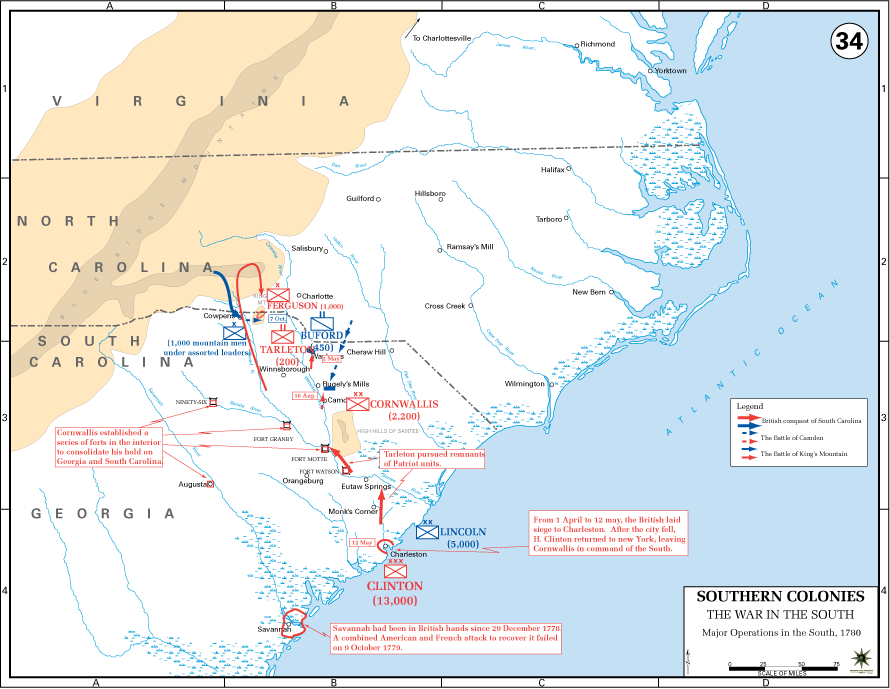
\includegraphics[height=5in]{gfx/Nicholson3}
\end{center}
\caption{Major operations in the South, 1780 \cite[Map 34]{web:USMA:map34}}
\label{Nicholson3}
\end{figure}

The British army “established garrisons at Georgetown and Beaufort as well as
the capital along the coast, and at Camden, Rocky Mount, and Ninety Six to
shield the northern border of the province and watch over the interior”
\cite[p.10]{weigley_partisan_1970}.  (See Fig. \ref{Nicholson3}) Settlements in
the far west put the British in contact with the “friendly, anti-Revolutionary
Creek and Cherokee Indians and threatened American settlements beyond the
mountains” \cite[p.10]{weigley_partisan_1970} 

In June 1780, General Clinton returned to New York leaving General Earl
Cornwallis in Command.  General Cornwallis was a proven British field commander
with a wealth of experience in the American area of operations.  General
Cornwallis commanded a force of about 3,000 men
\cite[p.51]{woodward_comparative_2002}.  With this
relatively small force, he was to achieve the campaign objectives given to him
by General Clinton.  

General Clinton gave Cornwallis instructions to defend Charleston above all else
because of its logistical and political importance.  He was to maintain gains in
Georgia and establish control over South Carolina eventually move into North
Carolina.  Clinton also expected Cornwallis “to provide some 3,000 troops for
operations in the Chesapeake region at some indefinite time in the future”
\cite[p.51]{woodward_comparative_2002}.  

In order to achieve his objectives Cornwallis would have to raise Loyalist
militias.  The British Army required the use of Loyalist militias as a means to
reach the Southern Campaign objectives.  Even with sizable Loyalist militias it
would be nearly impossible to achieve all of the above campaign objectives with
a force of 3,000 troops augmented by Loyalist militias.   In order to have
achieved the campaign objectives listed above the British needed to win the
hearts and minds of the people.  The British consistently alienated the neutral
American or pro British citizenry through failed policies forcing these
non-players into opponents.  

The British exercised poor decision making when dealing with the treatment of
the American populations following the fall of Charleston.  An example of failed
policy when dealing with paroled prisoners from American militias came just
prior to General Clinton’s handover to General Cornwallis.  The following
passage describes the change in policy:

\begin{quote} “Just before departing Clinton announced abandonment of the system
  whereby rebels were regarded as under parole and substituted a policy which
  offered full civil rights to all who showed complete loyalty, but punishment
  as enemies to any who did not; this compulsion of a clear choice between
  loyalty and a return to rebellion, when many would have preferred a neutrality
  which might have served Clinton just as well, perversely helped drive men back
  into rebellion” \cite[p.12]{weigley_partisan_1970}.  \end{quote} 

This British policy for dealing with prisoners on parole unnecessarily increased
the combat power of the Americans.

Another example of failed policy was when British leaders allowed their troops
to loot and commit crimes against civilians.  This drove otherwise neutrals to
side with the “Patriot cause” \cite[p.13]{weigley_partisan_1970}.   The Scotch-Irish of the
backcountry were “driven into rebels arms” by a British policy allowing
hostility towards the Presbyterian church \cite[p.13]{weigley_partisan_1970}.  Presbyterian
churches were burned simply because they were thought to harbor rebels.  

The backcountry of South Carolina was the frontier and contained a
disproportioned number of Loyalists.  Backcountry folks distrusted “anything the
low country did; and because the lowland planters led the Revolutionary
movement, the backcountry tended to distrust the Revolution as an event
calculated simply to render them still more subservient to the planter’s
political power.  By the time the war began, about half the population of South
Carolina resided in the backcountry, though with much less than half the
membership of the assembly “\cite[p.11]{weigley_partisan_1970}.  

This disproportionate number of Loyalists in the upcountry helped inspire the
British concept of the Southern Campaign.  Instead of exploiting this wedge and
using these inlanders to fill the ranks of Loyalist militias in order to reach
British campaign objectives, failed British policy forced these neutral or
pro-British populations to rise against the British.  Native Americans were also
poorly integrated into British strategy to achieve campaign objectives.  Before
the Southern Campaign, the Cherokee also opposed the Revolution, but they did
“not coordinate their actions with either the Loyalists or the British, and in
1776, Williamson led an expedition against them which considerably stunted their
ability to make trouble” \cite[p.12]{weigley_partisan_1970}.

After the fall of Charleston many of these failed British policies led to a
rising resistance.  Many alienated groups as well as those already opposing
British rule began taking up arms.  However, these resistance groups were poorly
planned and organized with no real campaign objectives except  “self
preservation and revenge” \cite[p.14]{weigley_partisan_1970}.  The pockets of resistance utilized
guerilla warfare to fight the British.  

Thomas Sumter, “the Gamecock”, and other rebels moved on horseback moved on
horseback moving much too fast for larger British forces to catch them
\cite[p.15]{weigley_partisan_1970}.  They relied on surprise and guerilla warfare-like tactics
\cite[p.15]{weigley_partisan_1970}.  These terrorist attacks forced the British to “disperse
their forces over wider and wider areas and thus made them still more
vulnerable” \cite[p.16]{weigley_partisan_1970}.  British failed policy gave way to a
strengthened informal resistance further occupying and weakening British forces
thus allowing the Continental Congress time to re-establish a more traditional
Army in the Southern
Department.

In July 1780 Major General Horatio Gates took command of the Southern Department
due to Major General Baron Jean De Kalb being born abroad.  The command
consisted of about 4,200 Continentals and militiamen \cite[p.21]{moncure_cowpens_1996}.  This
force was adequate to annoy and harass the British but not destroy them.
Instead of utilizing his forces in this manner, Gates returned to traditional
warfare before his force was ready and trained.  His first objective was to take
Camden with a direct straight advance to the city. 

On August 16, 1780, the Continental Army met the British Army in an open field
in Camden. (See \ref{Nicholson2})

  The British had more than 2,000 men and Gates had
about 3,000 \cite[p.19]{weigley_partisan_1970}.  Quantitatively the Americans were not outmatched,
but qualitatively the British had a significant advantage.  The British won the
battle quite easily with Gates leading the retreat with about 700 Americans
surviving the battle \cite[p.21]{weigley_partisan_1970}.  De Kalb died with the “Maryland and
Delaware Continentals, still leading them in a counterattack after everyone else
had fled” \cite[p.21]{weigley_partisan_1970}.  After Camden, Cornwallis prepared to move into North
Carolina by “sending word to Loyalists in that state to begin assembling and
seizing Patriot stores” \cite[p.27]{woodward_comparative_2002}.

Virtually, all formal organized Continental forces were destroyed leaving only
the informal resistance to survive.  Once again, these pockets of resistance
utilized guerilla warfare to annoy and harass the enemy quite successfully.  A
leader of one of these resistance groups was Colonel Francis Marion.  Marion
“the Swamp Fox” and his force of disreputables rose from the coastal swamps and
caused enough trouble to force Tarleton to pursue him.  Tarleton found pursuing
Marion so useless that he decided to pursue Sumter instead.  Tarleton supposedly
said, “Let us go back and we will find the gamecock.  But as for this damned old
fox, the devil himself could not catch him!” \cite[p.23]{weigley_partisan_1970}

Another example of British policy was the treatment of neutral civilian
population at Kings Mountain.  The negative treatment drove them to become part
of the rebellion against British forces when no organized Southern Continental
forces existed.  Major Patrick Ferguson of the 71st Highlanders “threatened the
settlements beyond the Appalachians that they had better make peace or be
punished” \cite[p.24]{weigley_partisan_1970}.  His threats motivated 1400-1800 mountain men to
rise up in arms against him.  The Mountain men “killed Ferguson and 157 of his
Loyalists and captured the rest, 163 badly wounded and 698 others” (Weigley,
p.25).  

Tarleton and “the Gamecock” met head to head for a final time at Blackstocks
Plantation on the Tyger River on November 20, 1780.  Both sides fought to a
stalemate and slipped away at night claiming victory.  Sumter was wounded during
the encounter, no longer being a significant force in the Southern Campaign. 

The informal resistance groups kept the British occupied, allowing the
Continentals to once again raise an army.  On December 2, 1780 Nathanael Greene
arrived at Charlotte, North Carolina to assume command \cite[p.22]{moncure_cowpens_1996}.
His combat experience included “participation in every major battle under
Washington between 1776 and 1779” (Babits, p.5).  Greene assumed command of a
force “2,457 strong, though with only 1,482 present and fit for duty, only 1,099
of the muster roll strength Continentals”  (Weigley, p.27).   However, Greene
described his force as being “wretched” and “distressed” and “starving with cold
and hunger, without tents and camp equipage” (Moncure, p.23). 

American strategy during the Southern Campaign was “disjointed”
\cite[p.60]{woodward_comparative_2002}. This was caused by a “series of leadership turnovers that
produced frequent changes to the strategic direction” (Woodward, p.61).  

\begin{quote} “Lack of continuity was exacerbated by a severe shortage of
  resources to conduct the campaign with.  The Southern department received
  little external assistance.  Each successive American commander had to figure
  out for himself how to mount an effort that would support the national
  military effort” \cite[p.61]{woodward_comparative_2002} \end{quote}

Washington's primary strategic goal for the Southern Campaign was to break the
British will to fight.  Lincoln and Gates both pursued strategies that were
destined to fail to reach their campaign objectives thus failing to accomplish
Washington’s strategic goal.  Both Lincoln and Gates pursued a conventional
campaign by seeking to engage the British in decisive battle.  Lincoln’s goal
was to prevent the British a “foothold in the South” and Gates’ goal was to push
the British “back to the sea” \cite[p.64]{woodward_comparative_2002}. 

Nathanael Greene’s time in command covered more time in the Southern campaign
than any other Commander of the Southern Department.  For this reason and his
overall success, his strategy and campaign objectives are the clearest for the
Americans during the Southern Campaign.  General Washington’s only guidance to
Nathanael Greene:  “Uninformed as I am of the enemy’s force in that quarter, of
our own, or of the resources, I can give you no particular instructions, but
must leave you to govern yourself entirely according to your own prudence and
judgement, and the circumstances in which you find yourself”
\cite[p.63]{woodward_comparative_2002}.

Greene’s campaign objectives were to avoid destruction of his force, raise
militia forces, and wear down Cornwallis.  However, he had to address logistical
concerns before he could begin to hope to reach his operational objectives.
General Greene knew that if his army was destroyed it would leave the Carolinas
without a formal Southern Department of the Continental Army for a third time.
This possible third destruction may have resulted in not being able to raise a
fourth army.  His primary responsibility as he saw it, was to be conservative
and maintain his army at all costs without taking great risks. Nathanael Greene
would not repeat the mistakes of his predecessors by fighting the British on
their terms.   Greene knew that the “strategic value of his army was in its
existence more than its ability to defeat its British counterpart”
\cite[p.66]{woodward_comparative_2002}.

\begin{figure}[h]
\begin{center}
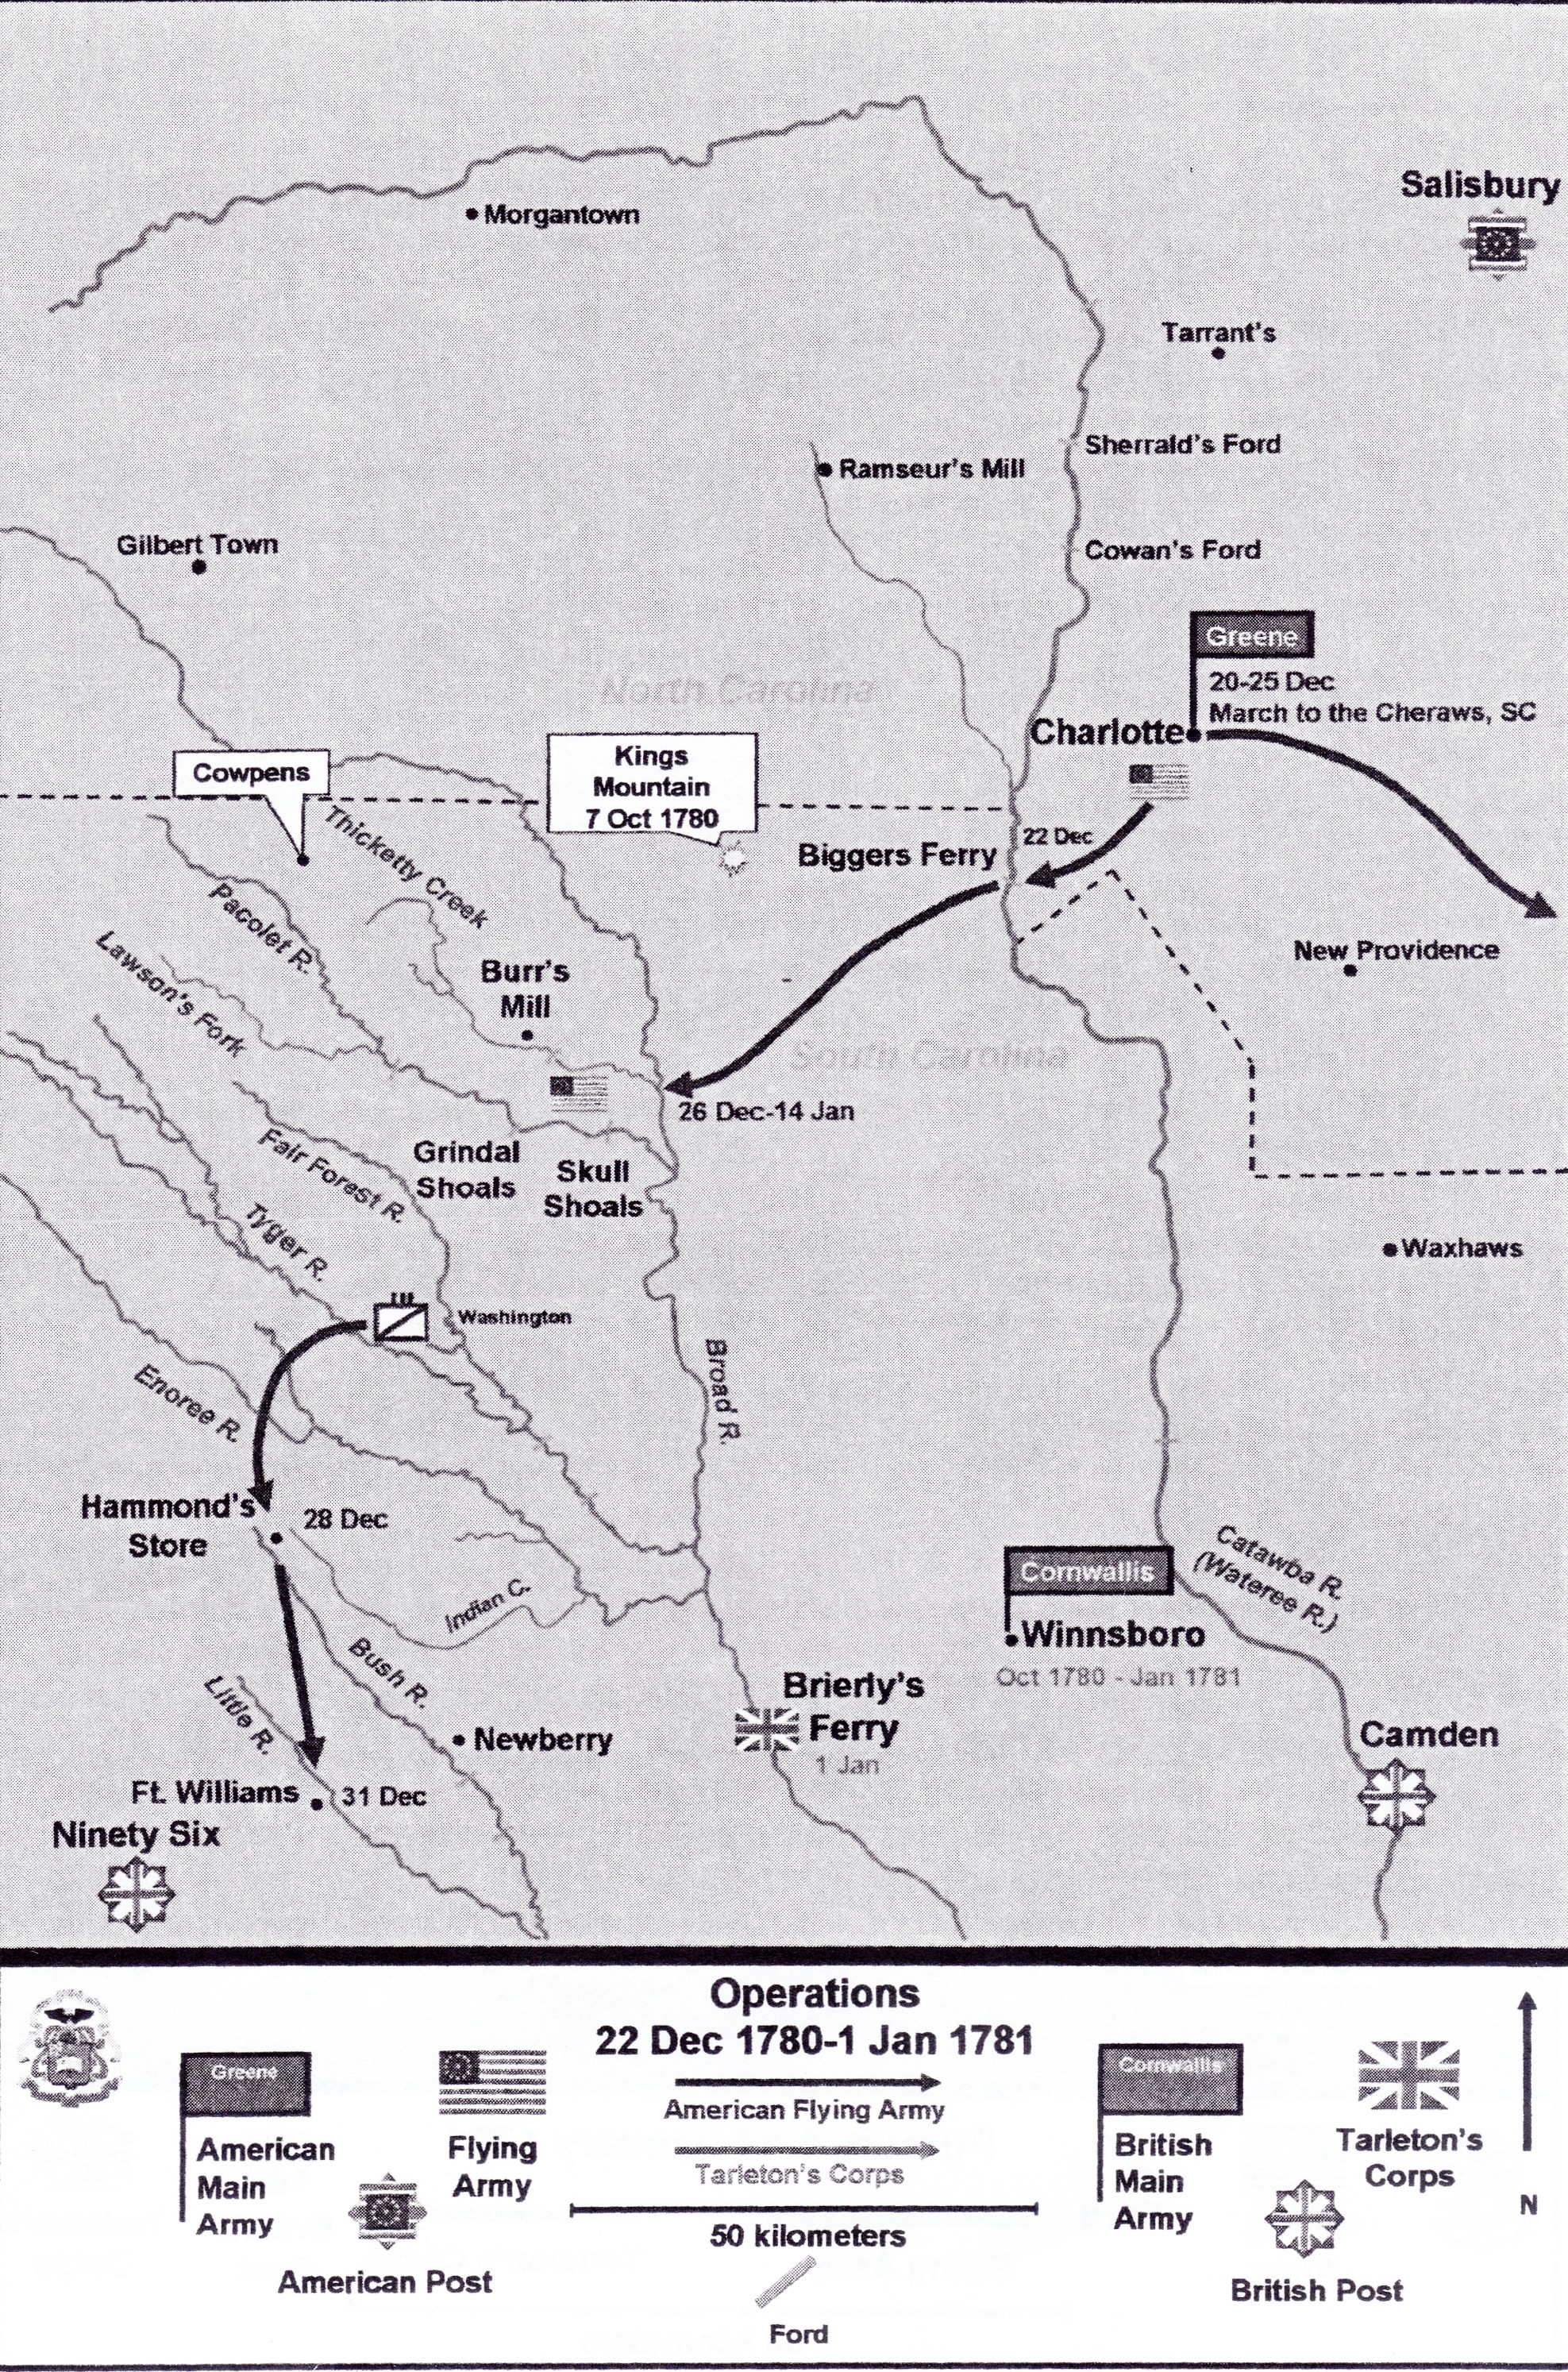
\includegraphics[height=5in]{gfx/Nicholson4}
\end{center}
\caption{Operational Actions 22 DEC 1780---01 JAN 1781 \cite[Tab D, Map 6]{rauch_battle_2007}}
\label{Nicholson4}
\end{figure}

Greene divided his army by moving his main force to Cheraws, South Carolina,
sending General Morgan West and Lieutenant Colonel Henry East to join Marion
with his operations on the coast (See Fig. \ref{Nicholson4}).  The combined
forces of Lee and Marion attacked Georgetown, South Carolina, on January 25,
1781.  This division of forces was done for logistical reasons.  Colonel Tadeusz
Kosciuszko had found “adequate supplies” in Cheraws for the main body
\cite[p.23]{moncure_cowpens_1996}.  By dividing his forces it lessened the number of soldiers
in one place, thus requiring fewer supplies from each location.  

Brigadier General Daniel Morgan led the smaller force of 600 was led south west
towards Ninety Six \cite[p.27]{weigley_partisan_1970}.  Greene’s orders to Morgan were to
conduct operations “either offensively or defensively, as your own prudence and
discretion may direct-acting with caution and avoiding surprises by every
possible precaution” \cite[p.27]{weigley_partisan_1970}.  On December 16, 1780, Morgan
received further guidance from Greene to conduct a “prudent campaign designed to
call attention to itself” \cite[p.24]{moncure_cowpens_1996}.  The guidance to Morgan was to
raise a militia, protect patriot settlements, improve the morale of the people
and “annoy the enemy in that quarter” \cite[p.24]{moncure_cowpens_1996}.  Finally, if
Cornwallis were to pursue Morgan he was to rejoin the main army.  

Morgan left Charlotte on December 21, and marched about 55 miles and encamped at
Grindal Shoals on Christmas Day on the Pacolet River.  Following Greene’s
guidance, Morgan raised militia forces augmenting his detachment to about 1,040
men \cite[p.28]{weigley_partisan_1970}.   The force included “320 of the stout Maryland and
Delaware Continentals and 60 to 100 Continental light dragoons, who could fight
either mounted or on foot, under William Washington” \cite[p.28]{weigley_partisan_1970}.   On
December 28, Washington’s Continental dragoons and militia numbering about 300
destroyed a Tory force of 150 at Hammond’s Store then moved south and burned
Fort William a short distance from Ninety Six \cite[p.8]{babits_devil_2001}. (See Nicholson
4)

\begin{figure}[h]
\begin{center}
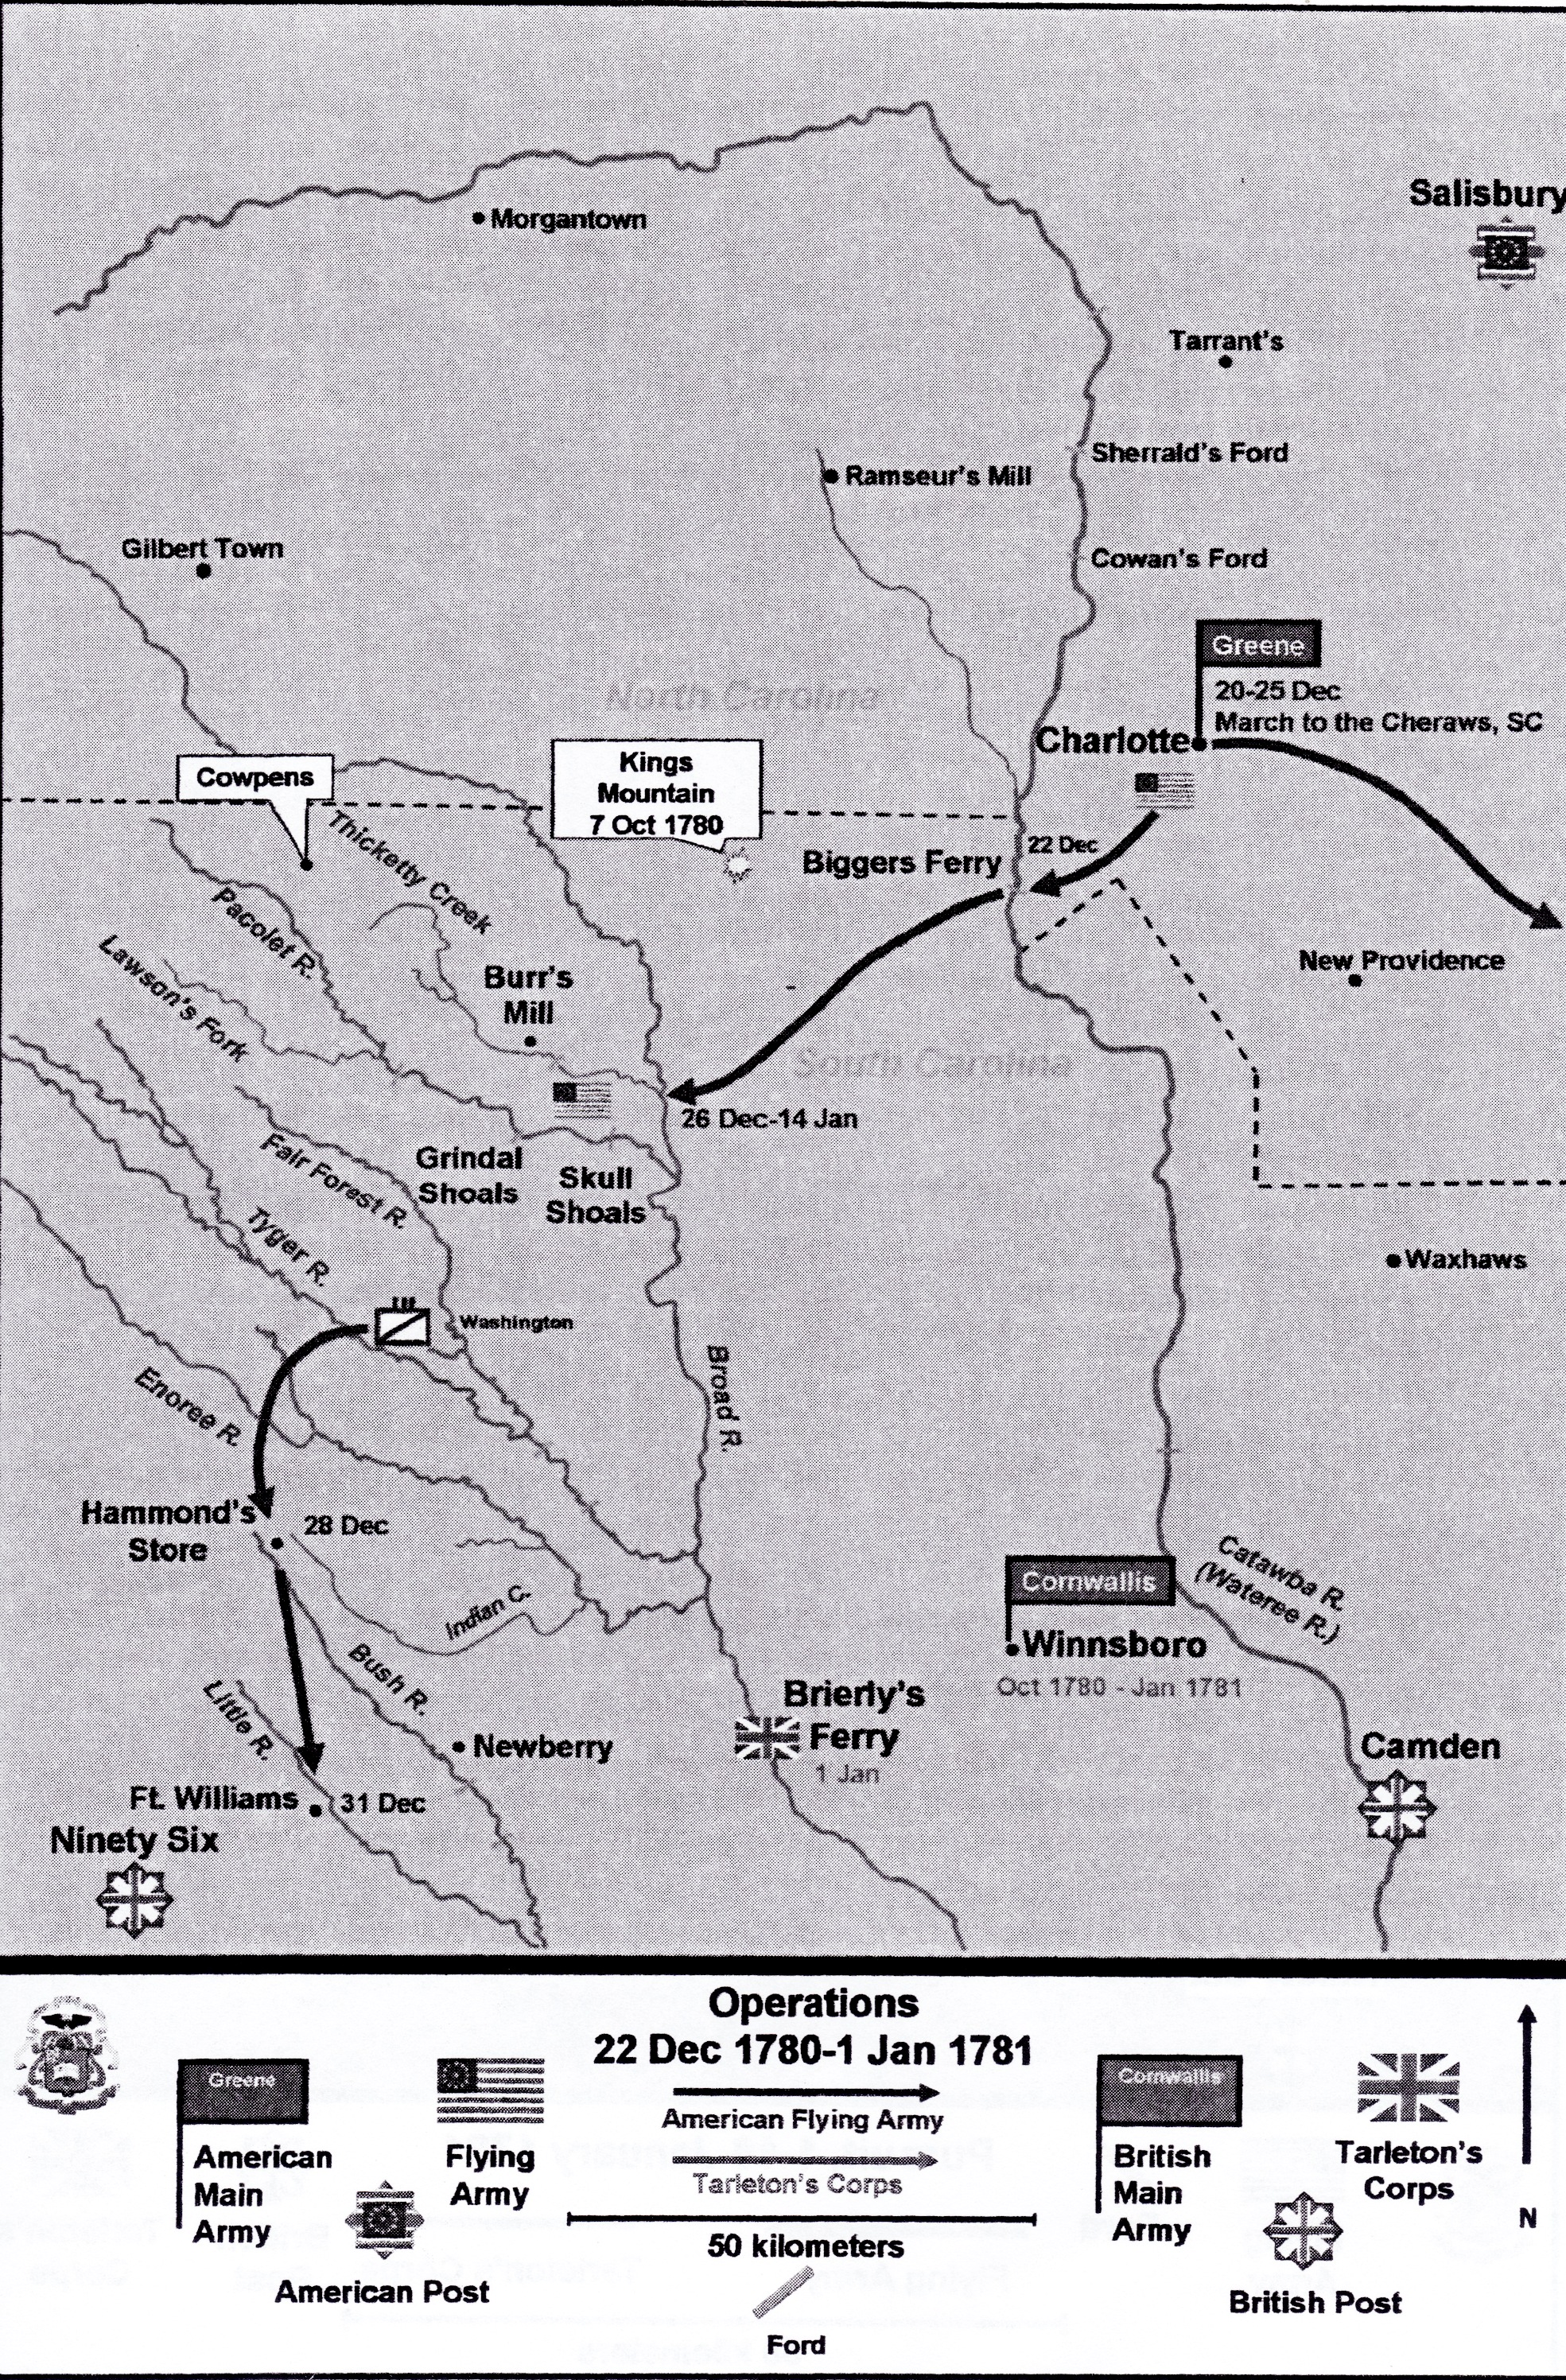
\includegraphics[height=5in]{gfx/Nicholson5}
\end{center}
\caption{Operational actions 1-16 Jan 1781 \cite[Tab D, Map 7]{rauch_battle_2007}}
\label{Nicholson5}
\end{figure}

Cornwallis could not direct his army toward either smaller Continental force
without exposing Charleston to attack or leaving the Western region vulnerable.
In response to Greene’s division of forces, Cornwallis was forced to divide his
own force, sending Tarleton with about 1,100 men, mixed cavalry and infantry to
deal with Morgan \cite[28]{weigley_partisan_1970}.   Tarleton moved westward and placed his force
roughly between Morgan and Ninety Six.  Tarleton then moved his forces northward
toward Morgan’s encampment at Grindal Shoals.   This move forced Morgan to move
his force North with Tarleton in pursuit. (See Fig. \ref{Nicholson5})


Tarleton aggressively pursued Morgan to an area known as Cowpens. 
(See Fig. \ref{Nicholson5}) This area is where these two forces would soon meet on the
field of battle.  The Battle of Cowpens itself will be discussed further in the
following sections of this paper.  The battle proved to be a turning point in
the Southern Campaign of the Carolinas in favor of the Americans. 

The British Army, from the beginning of the Southern Campaign planned and
prepared to conduct major combat operations rather than irregular warfare.
According to the United States Army Field Manual 3-0 Operations 2-12 (p.2-3), an
“operational theme describes the character of the dominant major operations
being conducted at any time within a land force commander’s area of operations.”
The two dominant operational themes throughout the Southern Campaign for both
sides were major combat operations and irregular warfare. 

In the beginning of the Southern Campaign at Charleston and later at Camden,
both sides followed the operational theme of conducting major combat operations.
Major combat operations can be simply described as army versus army.  The Army
Field Manual 3-0, 2-69 (p.2-13), describes successful major combat operations as
being able to:

\begin{quote} “…defeat or destroy the enemy’s armed forces and seize terrain.
  Commanders assess them in terms of numbers of military units destroyed or
  rendered combat ineffective, the level of enemy resolve, and the terrain
  objectives seized or secured. Major combat operations are the operational
  theme for which doctrine, including the principles of war, was originally
  developed.” \end{quote}

This operational theme describes why at the onset of the Southern Campaign and
later after Camden the Americans seemed destined to lose the campaign and
eventually the War for Independence.  The British had a marked advantage both in
quality and quantity for major combat operations.

The periods following the fall of Charleston and later Camden and to a lesser
degree throughout the entire Southern Campaign, the operational theme shifted
from major combat operations to irregular warfare for the Americans.  According
to \cite[\S 2-45, pp. 2-10]{fm3-0} FM 3-0, 2-45 (p.2-10), irregular warfare “is a violent struggle among state
and non state actors for legitimacy and influence over a population”.  The Field
Manual further describes irregular warfare as being amongst the people and
lacking the goal of military supremacy.  The FM 3-0, 2-46 (p.2-10) also
describes irregular warfare as avoiding, 

\begin{quote} “…a direct military confrontation. Instead, it combines irregular
  forces and indirect, unconventional methods (such as terrorism) to subvert and
  exhaust the opponent. It is often the only practical means for a weaker
  opponent to engage a powerful military force. Irregular warfare seeks to
  defeat the opponent’s will through steady attrition and constant low-level
  pressure.” \end{quote}

After General Greene assumed command of the Continental Army the operational
themes combined elements of both major combat operations as well as irregular
warfare, with an emphasis being on irregular warfare.  Irregular warfare was
conducted by pockets of resistance still conducting terrorist and insurgent
activities while Greene’s use of Morgan raising and training militias fell more
closely under unconventional warfare.  In addition, Green still used Morgan’s
force in more conventional means that would be classified as major combat
operations, such as Hammond’s Store and later at Cowpens.

For the most part, the British conducted operations that combined elements of
both major combat operations as well as irregular warfare, but focused primarily
on major combat operations while irregular warfare fell to the wayside.  The
British did conduct counter insurgency and counter terrorism activities but
usually with horrible consequences due to a lack of British policy towards the
American people, ultimately losing the battle for their hearts and minds.  The
focus by Cornwallis was major combat operations illustrated by his movement of
forces in pursuit of the next decisive battle.  

Ultimately, Nathanael Greene’s use of the combined operational themes of major
combat operations and irregular warfare, allowed him to achieve his Southern
Campaign operational objectives.  The British Army mainly employed major combat
operations with an inadequate force that was “overburdened by fighting a
conventional war and an unconventional war simultaneously” \cite[55]{woodward_comparative_2002}.  This
failed strategy by Cornwallis, resulted in his Southern Campaign operational
objectives not being met.

\subsection{The Context Within the Campaign}


\ldots

\subsection{Operational Themes (FM 3-0)}

\ldots

\subsection{Campaign Objectives}

\ldots

\subsection{Operational Events Leading to the Battle}

\ldots

\ctable[
  cap={Events leading to the Battle},
  caption={Operational events leading to the Battle of Cowpens.},
  pos=h,
  ]{>{\footnotesize}l>{\footnotesize}p{4in}}{}{							\FL
Year 		& Event 									\ML
~		& ~~~~~~~~~~~~~~~~~~~~~~~~~~~~~~~~~~~~~~~~~~~~~~				\NN
~ 		& ~ 										\LL
}

%---------------------
% % http://militaryhistory.about.com/od/americanrevolution/a/amrevcauses.htm
% Rise of Liberalism and Republicanism
% 
% As tensions regarding colonial lands and taxation increased during the 1760s
% and 1770s, many American leaders were influenced by the liberal and republican
% ideals espoused by Enlightenment writers such as John Locke. Key among Locke's
% theories was that of the ``social contract'' which stated that legitimate state
% authority must be derived from the consent of the governed. Also, that should
% the government abuse the rights of the governed, it was the natural
% responsibility of the people to rise up and overthrow their leaders. The ideas
% of Locke and other similar writers contributed to the American embrace of
% ``republican'' ideology in the years before the Revolution. Standing in
% opposition to tyrants, republicanism called for the protection liberty through
% the rule of law and civic virtue.
%--------------------------




